%%%%%%%%%%%%%%%%%%%%%%%%%%%%%%%%%%%%%%%%%%%%%%%%%%%%%%%%%%%%%%%%
%                                                              %
%                                                              %
% Macallyster S. Edmondson                                     %
%                                                              %
% ECE351-53                                                    %
%                                                              %
% Lab #6                                                       %
%                                                              %
% 03/01/2022                                                   %
%                                                              %
% Straightforward layout, broken into sections, uses many      %
% common libraries. Note, Hyperlinks are not highlighted.      %
%                                                              %
%%%%%%%%%%%%%%%%%%%%%%%%%%%%%%%%%%%%%%%%%%%%%%%%%%%%%%%%%%%%%%%%

%%%%%%%%%%%%%%%%%%%%%%%%%%%%%%%%%%%%%%%%%%%
%%% DOCUMENT PREAMBLE %%%
\documentclass[12pt]{report}
\usepackage[english]{babel}
%\usepackage{natbib}
\usepackage{url}
\usepackage[utf8x]{inputenc}
\usepackage{amsmath}
\usepackage{graphicx}
\graphicspath{{./images/}}
\usepackage{parskip}
\usepackage{fancyhdr}
\usepackage{vmargin}
\usepackage{listings}
\usepackage[hidelinks]{hyperref}
\usepackage{xcolor}
\usepackage[nodayofweek]{datetime}
\usepackage[section]{placeins}
\usepackage{pdfpages}
\definecolor{codegreen}{rgb}{0,0.6,0}
\definecolor{codegray}{rgb}{0.5,0.5,0.5}
\definecolor{codeblue}{rgb}{0,0,0.95}
\definecolor{backcolour}{rgb}{0.95,0.95,0.92}
\lstdefinestyle{mystyle}{
backgroundcolor=\color{backcolour},
commentstyle=\color{codegreen},
keywordstyle=\color{codeblue},
numberstyle=\tiny\color{codegray},
stringstyle=\color{codegreen},
basicstyle=\ttfamily\footnotesize,
breakatwhitespace=false,
breaklines=true,
captionpos=b,
keepspaces=true,
numbers=left,
numbersep=5pt,
showspaces=false,
showstringspaces=false,
showtabs=false,
tabsize=2
}
\lstset{style=mystyle}
\setmarginsrb{3 cm}{2.5 cm}{3 cm}{2.5 cm}{1 cm}{1 cm}{1 cm}{1.5 cm}
\title{Lab \#6 Report}
% Title
\author{Macallyster S. Edmondson}
% Author
\newdate{date}{03}{01}{2022}
\date{\longdate\displaydate{date}}
% Date
\makeatletter
\let\thetitle\@title
\let\theauthor\@author
\let\thedate\@date
\makeatother
\pagestyle{fancy}
\fancyhf{}
\rhead{\theauthor}
\lhead{\thetitle}
\lfoot{Page: \thepage}
\rfoot{\thedate}
\fancypagestyle{customplain}{ %Used for default pages with plain style to keep overall document consistency
  \fancyhf{}
  \renewcommand{\headrulewidth}{0pt} %Remove bar from top of page
  \lfoot{Page: \thepage}
}
\fancypagestyle{titlepage}{ %Used for default pages with plain style to keep overall document consistency
  \fancyhf{}
  \renewcommand{\headrulewidth}{0pt} %Remove bar from top of page
  \cfoot{\thedate}
}
\fancypagestyle{customblank}{ %Used for default pages with plain style to keep overall document consistency
  \fancyhf{}
  \renewcommand{\headrulewidth}{0pt} %Remove bar from top of page
}
%%%%%%%%%%%%%%%%%%%%%%%%%%%%%%%%%%%%%%%%%%%%
\begin{document}
%%%%%%%%%%%%%%%%%%%%%%%%%%%%%%%%%%%%%%%%%%%%%%%%%%%%%%%%%%%%%%%%%%%%%%%%%%
%%%%%%%%%%%%%%%
\begin{titlepage}\thispagestyle{titlepage}
\centering
%\vspace*{0.5 cm}

\includegraphics[scale = 0.12]{univ-logo.png}\\[1.0 cm]
%University of Idaho
\begin{center}    \textsc{\Large   ECE 351 - Section \#53 }\\[2.0 cm]
\end{center}% University Name

%Lab Report
\rule{\linewidth}{0.2 mm} \\[0.4 cm]
{ \huge \bfseries \thetitle}\\
\rule{\linewidth}{0.2 mm} \\[0.5 cm]
\textsc{\Large Partial Fraction Expansion Using Python }\\[1.5 cm] % Course 
\begin{minipage}{0.4\textwidth}
\begin{flushleft} \large
\emph{Submitted To:}\\
Kate Antonov\\ \small
University of Idaho\\
kantonov@uidaho.edu\\
\hfill
\end{flushleft}
\end{minipage}~
\begin{minipage}{0.4\textwidth}
\begin{flushright} \large
\emph{Submitted By :} \\
\theauthor \\ \small
University of Idaho\\
edmo7033@vandals.uidaho.edu\\
\href{http://github.com/mac-edmondson}{github.com/mac-edmondson}\\
\end{flushright}
\end{minipage}\\[2 cm]
\vfill
\end{titlepage}
%%%%%%%%%%%%%%%%%%%%%%%%%%%%%%%%%%%%%%%%%%%%%%%%%%%%%%%%%%%%%%%%%%%%%%%%%%
%%%%%%%%%%%%%%%
\tableofcontents\thispagestyle{customplain}
\pagebreak
%%%%%%%%%%%%%%%%%%%%%%%%%%%%%%%%%%%%%%%%%%%%%%%%%%%%%%%%%%%%%%%%%%%%%%%%%%
%%%%%%%%%%%%%%%
\renewcommand{\thesection}{\arabic{section}}
\section{Introduction}
The goal of this weeks lab was to use the \texttt{scipy.signal.residue()} function to perform partial fraction expansion within Python. I found this lab very useful
and was able to apply the methods taught in this lab to double check homework submissions. Before the lab, a preliminary was completed which can be found attached to
this report. The preliminary directly correlates to Part 1 (\ref{Section: Part1}) of this lab. Yet again, this lab was completed using \textit{Python} through the \textit{Spyder-IDE}. 
The packages used in the completion of this lab were \texttt{numpy} for 
definitions of mathematical functions, \texttt{matplotlib.pyplot} to plot outputs of functions, and \texttt{scipy.signal} to perform the step response and find the 
partial fraction expansion of a polynomial. 

All code for this lab, including this report, can be found on \href{http://github.com/mac-edmondson}{my Github}.
\section{Equations}\label{section: eq}
The equations used within this lab are shown in this section. The equations will be referenced by number throughout the rest of the report.
\begin{equation}\label{eq: 1}
  \begin{aligned}[c]
    y''(t) + 10y'(t) + 24y(t) = x''(t) + 6x'(t) + 12x(t)\\
  \end{aligned}
\end{equation}
\begin{equation}\label{eq: 2}
  \begin{aligned}[c]
    y^{(5)}(t) + 18y^{(4)}(t) + 218y^{(3)}(t) + 2036y^{(2)}(t) + 9085y^{(1)}(t) + 25250y(t) = 25250x(t)
  \end{aligned}
\end{equation}

\section{Methodology}
\subsection{Lab: Part 1}\label{Section: Part1}
Part 1 of this lab was very simple. The code implemented for this part of the lab plots the step response based on the hand-calculated time-domain function
based on the differential equation \eqref{eq: 1} found in
the preliminary, seen in \ref{section: Attachments}, as well as the step response found using the \texttt{scipy.signal.step()} function. Additionally, we used the
\texttt{scipy.signal.residue()} function to find the R, P, \& K Partial Fraction Expansion results of Y(s), again seen in \ref{section: Attachments}.

Below can be seen the code implementation of the tasks carried out in Part 1 of this lab.

\begin{lstlisting}[language=Python, basicstyle=\footnotesize]
  #PART 1
  #1/2
  def y(t) :
    h = (1/2 - 1/2 * np.exp(-4*t) + np.exp(-6*t)) * ss.u(t)
    return h

  system = ([1, 6, 12], [1, 10, 24])

  t = np.arange(0, 2 + step_size, step_size)
  y1 = y(t)        

  tout, y2 = spsig.step(system, T=t);

  #Plot...

  #3

  b = [0, 1, 6, 12]
  a = [1, 10, 24, 0]

  R, P, K = spsig.residue(b, a)

  print("Part 1:")
  print("Residue of Poles (same order as presented below): \n", R, "\n\nPoles in ascending order of mag.:\n", P, "\n\nCoefficent of Direct Polynomial Term: \n", K)
\end{lstlisting}

\subsection{Lab: Part 2}\label{section: Part2}
In Part 2 of this lab, we used the \texttt{scipy.signal.residue()} function to perform a PFE expansion on a function that would be difficult to analyze by hand, in this
case Equation \eqref{eq: 2}.
Additionally, I made a function to implement the Cosine Method to plot the time-domain output of the solution to the differential equation. This was further verified
using the \texttt{scipy.signal.step()} with the system based on Equation \eqref{eq: 2}. The printed output of the PFE result was also printed. 

Below can be seen the code implementation of the tasks carried out in Part 2 of this lab.
\begin{lstlisting}[language=Python, basicstyle=\footnotesize]
  #PART 2

  #1

  b = [0,   0,   0,    0,   0,    0, 25250]
  a = [1, 18, 218, 2036, 9085, 25250, 0]

  R, P, K = spsig.residue(b, a)

  print("Part 2:")
  print("Residue of Poles (same order as presented below): \n", R, "\n\nPoles in ascending order of mag.:\n", P, "\n\nCoefficent of Direct Polynomial Term: \n", K)


  #2
  def cos_mthd(R, P, t):
      y = 0;
      for i in range(0, len(R)):
          k_mag = np.absolute(R[i])
          k_ang = np.angle(R[i])
          alpha = np.real(P[i])
          omega = np.imag(P[i])
          y += k_mag*np.exp(alpha*t)*np.cos(omega*t + k_ang)*ss.u(t)
      return y

  def y_s1(t):
      y = (626.375/4)*np.exp(-3*t)*np.sin(4*t-np.deg2rad(156.615))*ss.u(t)
      return y
      
  def y_s2(t):
      y = (186.75/10)*np.exp(-1*t)*np.sin(10*t - np.deg2rad(143.723))*ss.u(t)
      return y

  def y_t(t):
      y = (1 * ss.u(t)) - (0.215*np.exp(-10*t)*ss.u(t)) + y_s1(t) + y_s2(t)
      return y

  #3
  system = ([0,   0,   0,    0,   0,  25250], [1, 18, 218, 2036, 9085, 25250])

  t = np.arange(0, 4.5 + step_size, step_size)
  # y1 = y_t(t) 
  y1 = cos_mthd(R, P, t)       

  tout, y2 = spsig.step(system, T=t);

  #Plot...
\end{lstlisting}

\section{Results}\label{section: Results}
The results of this lab are very straightforward. The implementation of all functions worked as expected and the results are as expected.

The deliverables for Parts 1 \& 2 of this lab can be seen in Figures \ref{fig: p1t1}, \ref{fig: p1t2}, \ref{fig: p2t1} \& \ref{fig: p2t2}, below.
\\
\begin{figure}[h!]
  \centering
  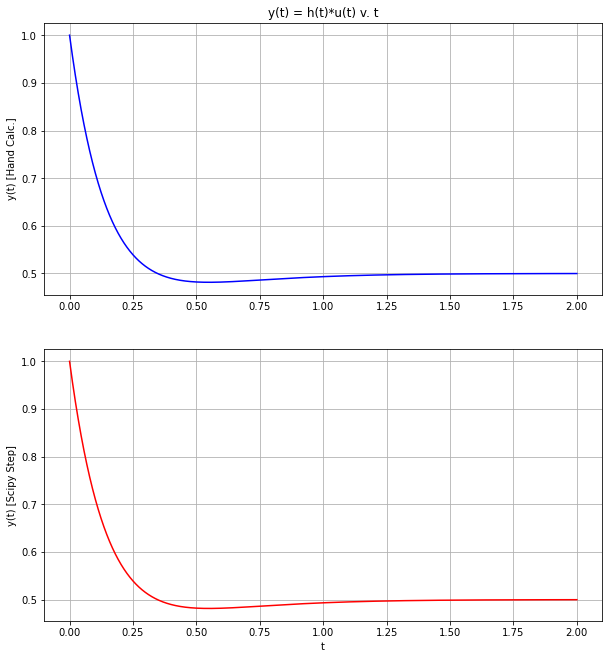
\includegraphics[scale=0.5]{p1t1.png}
  \caption{Part 1, Task 1}
  \label{fig: p1t1}
\end{figure}
\begin{figure}[h!]
  \centering
  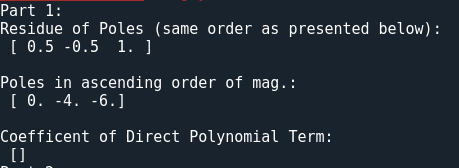
\includegraphics[scale=0.5]{p1t2.png}
  \caption{Part 1, Task 2}
  \label{fig: p1t2}
\end{figure}
\begin{figure}[h!]
  \centering
  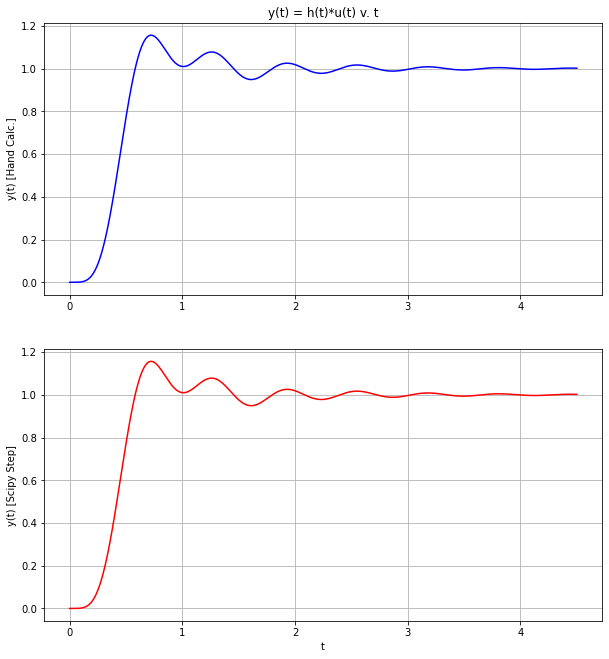
\includegraphics[scale=0.5]{p2t1.png}
  \caption{Part 2, Task 1}
  \label{fig: p2t1}
\end{figure}
\begin{figure}[h!]
  \centering
  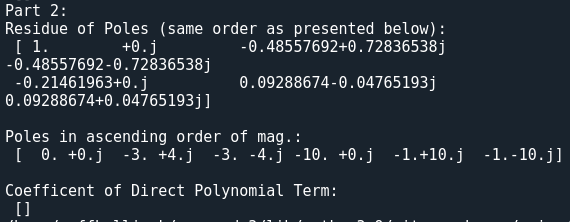
\includegraphics[scale=0.5]{p2t2.png}
  \caption{Part 2, Task 2}
  \label{fig: p2t2}
\end{figure}
\section{Error Analysis}\label{section: ErAn}
No sources of error were seen throughout this lab, though I did run into trouble while completing Part 2 of this lab. At first, I had decided to attempt to solve
Equation \eqref{eq: 2} by hand using the sine method but was unsuccessful. I then followed the advice of the Lab TA and lab sheet and decided to implement a function
which took the outputs of the \texttt{scipy.sig.residue} function to plot the time-domain response of the equation, as seen in \ref{section: Part2}.
\section{Questions}
\begin{enumerate}
  \item The cosine method can still be used for a non-complex pole-residue term is due to the fact that for a non-complex pole-residue term, $\omega$ in p is 0
  and you are just then left with the coefficient of a PFE term times $e^{\alpha t}$. 
  \item This lab and its tasks were very concise in what is expected for deliverables. The preliminary work fit perfectly with not only what the lab was about,
  but also what we have been covering in class.
\end{enumerate}
\section{Conclusion}
In conclusion, I feel this lab was very successful. The implementation of the code in this lab was quite simple and I really enjoyed seeing how accurate the 
\texttt{scipy.signal} functions were as compared to hand calculated functions. All in all, I am very satisfied with what this lab has taught me and feel it was an excellent use of time.
\newpage
\thispagestyle{customblank}
\section{Attachments}\label{section: Attachments}
\centering\begin{enumerate}
  \item Pre-Lab
\end{enumerate}
\vspace*{\fill}

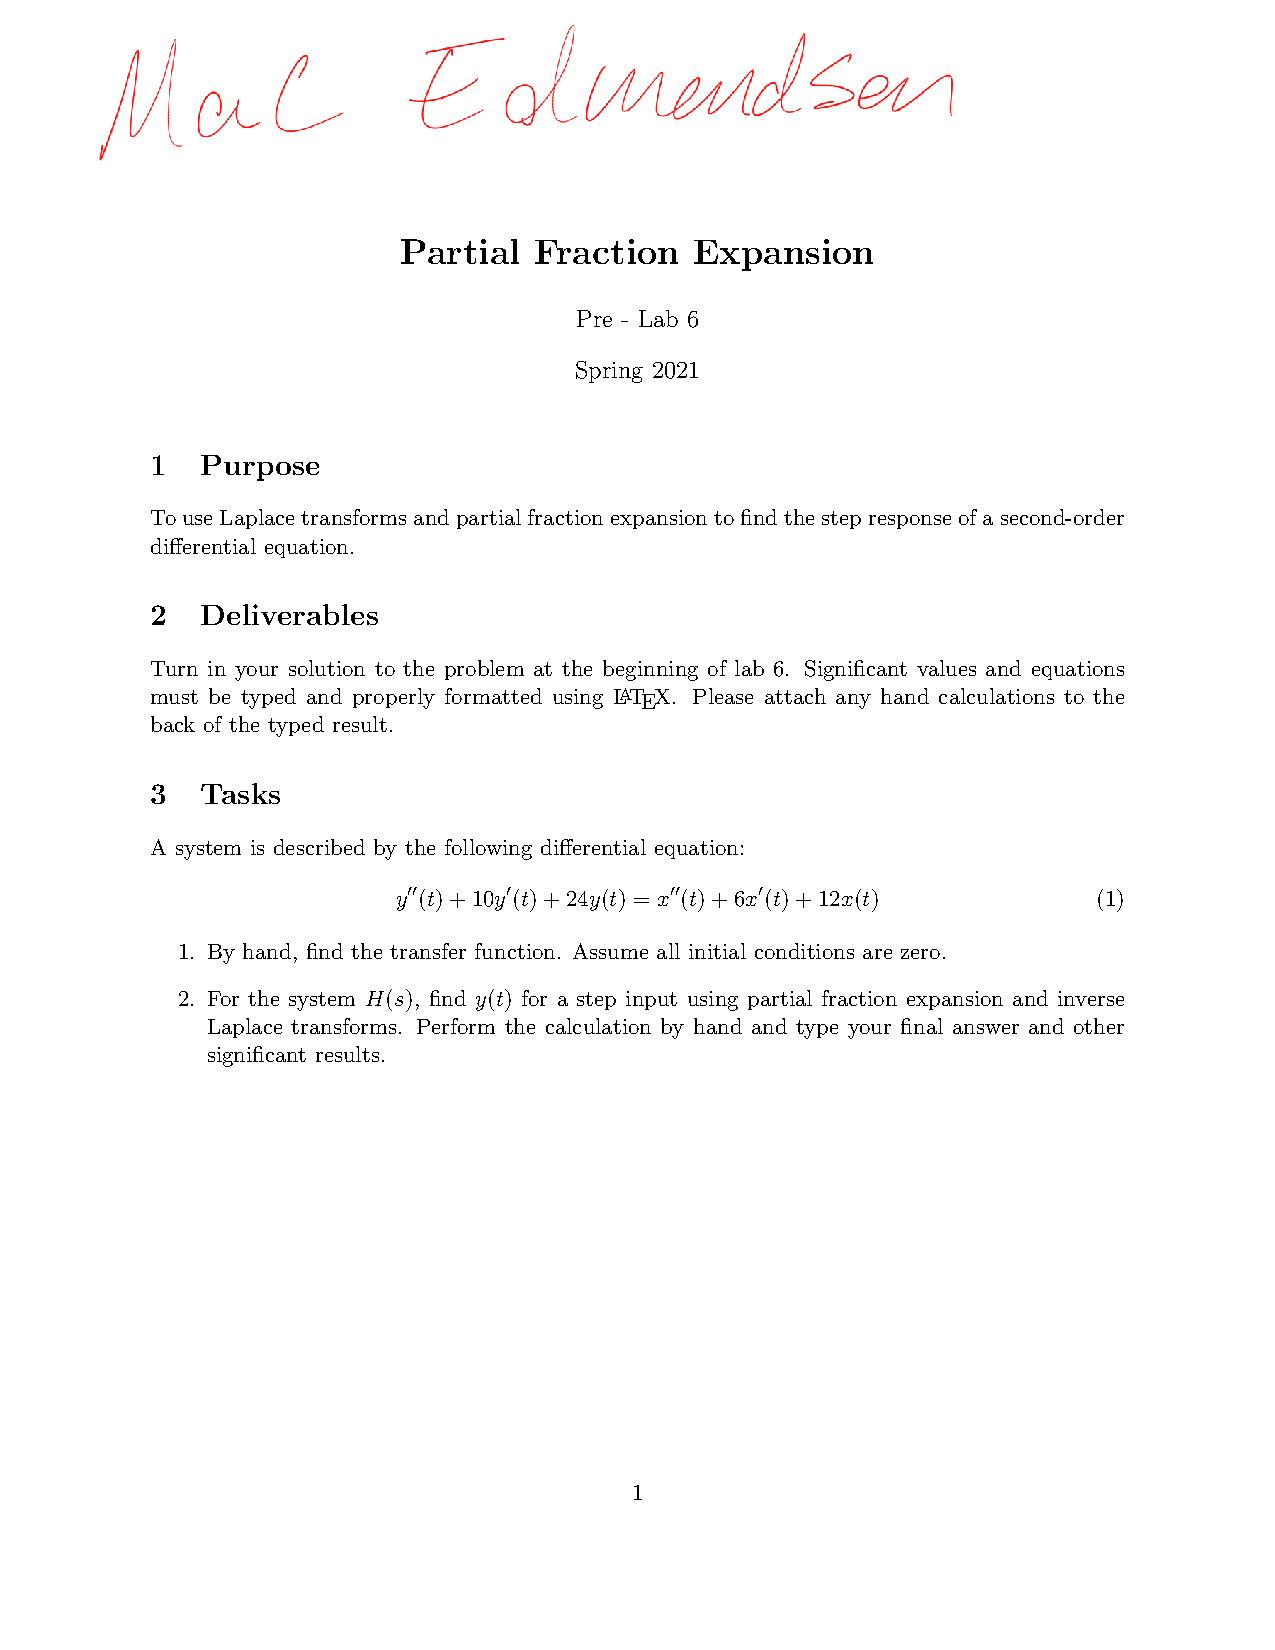
\includepdf[pages=-, offset=1in -1in]{./attachments/lab6_pre.pdf}
% \includepdf[pages=3, offset=1in -1in]{./attachments/lab5.pdf}

% \begin{thebibliography}{111} 
% \thispagestyle{customplain}

% \end{thebibliography}
\end{document}
%This template was created by Roza Aceska.